
\begin{figure}[htbp]
    \centering
    \tikzset{%
        neuron/.style={
                circle,
                draw,
                minimum size=8mm
            },
        neuronlabel/.style={
                circle=none,
                draw=none,
                text height=0.7cm,
            },
        edgelabel/.style={
                circle=none,
                draw=none,
                text height=0.8cm,
            },
        conditioned/.style={
                fill=gray
            },
    }
    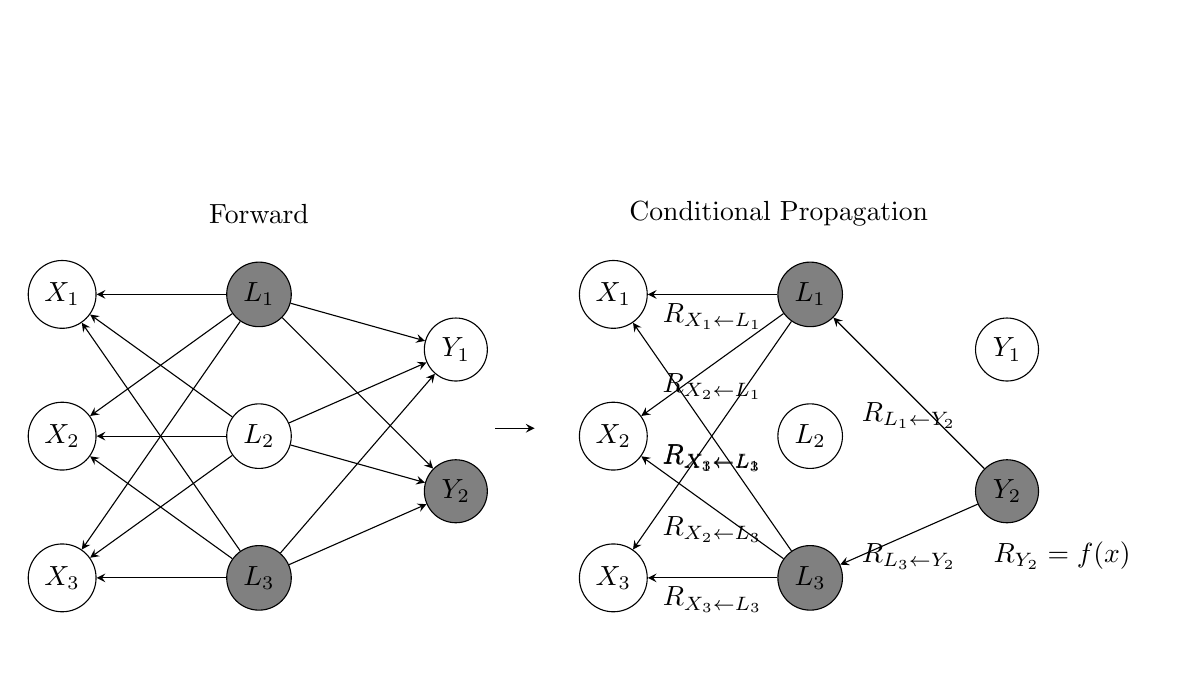
\begin{tikzpicture}[>=stealth,
            every node/.style={ draw, minimum size=8mm, align=center},]

        % First layer
        \foreach \x in {1,2,3} {
                \node [neuron] (X\x) at (0,{-\x* 1.8}) {$X_\x$};
            }
        \node [edgelabel]  (ti1) at (2.5,-0.5) {Forward};
        % Second layer
        \foreach \x in {1,2,3}{
                \pgfmathparse{\x==1 || \x ==3}
                \ifnum \pgfmathresult=1
                    \node  [neuron, conditioned]  (L\x) at (2.5,{-\x* 1.8}) {$L_\x$};
                \else
                    \node  [neuron]  (L\x) at (2.5,{-\x* 1.8}) {$L_\x$};
                \fi
            }

        % Last layer
        \foreach \x in {1,2} {
                \ifnum \x = 2
                    \node [neuron, conditioned]  (Y\x) at (5,{-\x* 1.8 - 0.7}) {$Y_\x$};
                    %\node [neuronlabel] at (Y\x.south) {$R_{Y_\x} = f(x)$};
                \else
                    \node  [neuron]  (Y\x) at (5,{-\x* 1.8 - 0.7}){$Y_\x$};
                \fi
            }

        % Connect nodes
        \foreach \y in {1,2,3}
        \foreach \x in {1,2,3}{
                \ifnum\x=\y
                    \draw[<-] (X\x) -- (L\y);
                    %node[midway, edgelabel] {$R_{X_\x  \gets L\y}$};
                \else
                    \pgfmathparse{2 > \x-\y && 2 > \y-\x}
                    \ifthenelse{\pgfmathresult=1}{\draw[<-] (X\x) -- (L\y);}{}
                \fi
            }
        \foreach \x in {1,2,3}
        \foreach \y in {1,2}
        \draw[->] (L\x) -- (Y\y);

        \draw[->] (5.5,-3.5) -- (6,-3.5);

        % OTHER GRAPH
        % First layer
        \foreach \x in {1,2,3} {
                \node [neuron] (X\x) at (7,{-\x* 1.8}) {$X_\x$};
            }

        % Second layer
        \node [edgelabel]  (ti2) at (9.1,-0.5) {Conditional Propagation};
        \foreach \x in {1,2,3}{
                \pgfmathparse{\x==1 || \x ==3}
                \ifnum \pgfmathresult=1
                    \node  [neuron, conditioned]  (L\x) at (9.5,{-\x* 1.8}) {$L_\x$};
                \else
                    \node  [neuron]  (L\x) at (9.5,{-\x* 1.8}) {$L_\x$};
                \fi
            }

        % Last layer
        \foreach \x in {1,2} {
                \ifnum \x = 2
                    \node [neuron, conditioned]  (Y\x) at (12,{-\x* 1.8 - 0.7}) {$Y_\x$};
                    \node [neuronlabel] at (12.7,{-\x* 1.8 - 1.3}) {$R_{Y_\x} = f(x)$};
                \else
                    \node  [neuron]  (Y\x) at (12,{-\x* 1.8 - 0.7}){$Y_\x$};
                \fi
            }

        % Connect nodes
        \foreach \y in {1,3}
        \foreach \x in {1,2,3}{
                \pgfmathparse{2 > \x-\y && 2 > \y-\x}
                \ifthenelse{\pgfmathresult=1}{\draw[<-] (X\x) -- (L\y)  node[midway, edgelabel] {$R_{X_\x  \gets L_\y}$};}{}
            }
        \foreach \x in {1,3}
        \foreach \y in {2}
        \draw[<-] (L\x) -- (Y\y) node[midway,align=center, edgelabel] {$R_{L_\x  \gets Y_\y}$};
    \end{tikzpicture}

    \caption[CRP Intuition]{\textbf{CRP Intuition:} Left side: simple neural network forward pass with input layer X, one hidden layer L and output layer Y. Conditioning set $\theta = \{L_1, L_3, Y_2\}$ \\ Right side: only the relevance of the neurons matching the conditioning set is propagated back \\
        Result at input pixel $R_{X_2} = \sum_{j}  R_{X_2 \gets L_j} =  \sum_i \sum_{j} \cdot \frac{a_i w_{ij}}{\sum_h a_h w_{hj}} R_j \dots$ }
    \label{fig:crp_example_condition}
\end{figure}
